\chapter{The Locate step}
\label{chap:locate}

\newcommand{\locateimgsize}{0.9\textwidth}

The task of the Locate step consists in extracting the positions of the bubbles in pixel coordinates, independently for each frame of each camera.

\section{State of the art}
TODO
\section{Requirements}

\subsection{Input}
The Locate step receives as input the videos captured by the cameras, frame by frame.
The images are pre-processed by the cameras: the background is removed, and the resulting image is binarized with a threshold, to have distinct white bubbles over a black background.
Figure~\ref{fig:locate:original} depicts an example input frame.

\begin{figure}
	\centerline{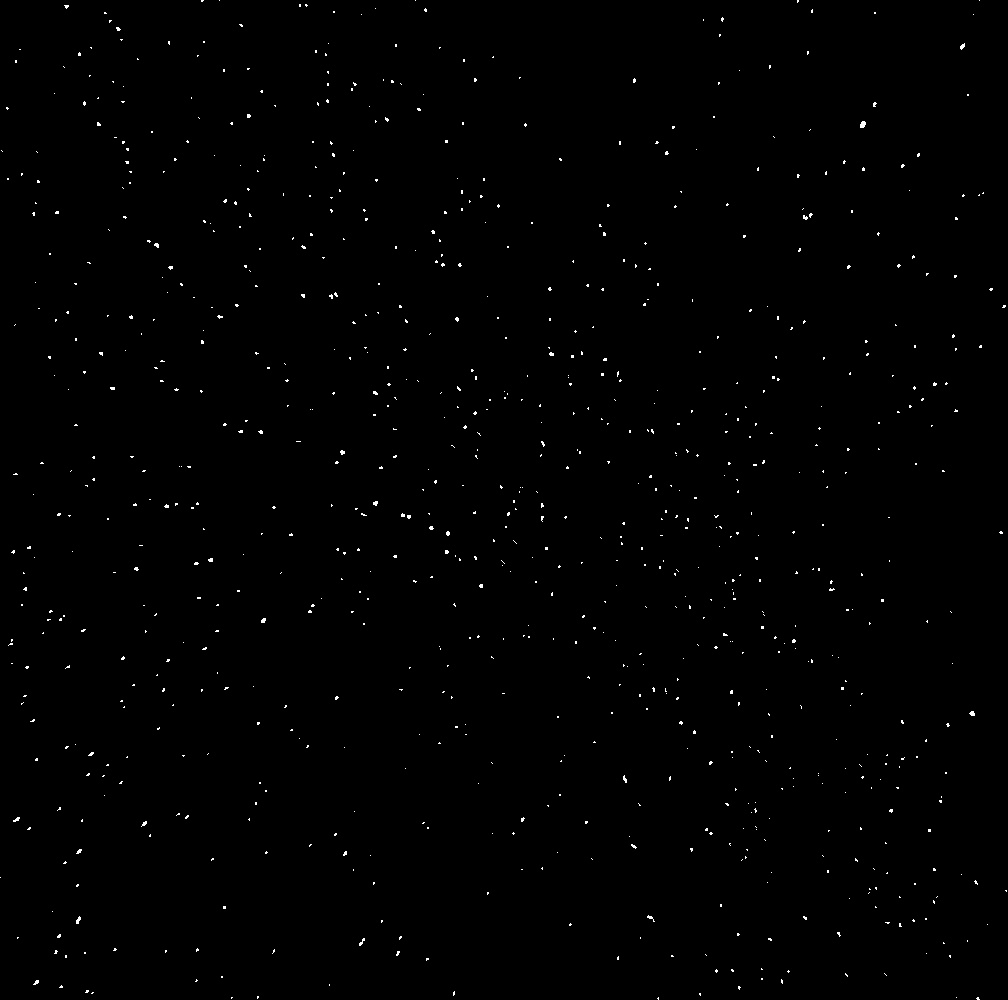
\includegraphics[width=\locateimgsize]{images/locate/_original-frame.png}}
	\caption{\centering An example of frame returned by the cameras}
	\label{fig:locate:original}
\end{figure}

\subsection{Output}

The output of the Locate step is a couple of \texttt{numpy} arrays.
An array called \texttt{positions} describes the coordinates of each bubble present in a frame. It is a four-dimensional, floating-point array, where \texttt{positions[C][F][B]} describes the $B$-th bubble of the $F$-th frame of camera $C$, in the form of an \texttt{(x, y[, area])} tuple.
Bubbles are ordered in a random, arbitrary way.

Due to \texttt{numpy} limitations, the array is pre-allocated of a fixed size: while the number of cameras is fixed, an upper limit on the number of frames and bubbles must be decided before execution.
Knowing which frames contain meaningful data is trivial, while it is not for the number of bubbles, that can change between frame and frame.
For this reason, a second array was introduced: \texttt{numTracers} is a two-dimensional, integer array.
\texttt{numTracers[C][F]} carries the information of how many tracers are valid inside the $F$-th frame of camera $C$.
The coordinates of the valid tracers will therefore be \texttt{positions[C][F][numTracers[C][F]]}.

\subsection{Speed}

When used on a setup of $N$ cameras with frame rate $f$ each, the Locate step would receive $N{\cdot}f$ independent frames each second.
To respect the real-time constraint, the Locate step would therefore need to operate at a minimum of $N{\cdot}f$ FPS.

When I did the analysis on the Locate step, the plan was to have 3 cameras working at 30 FPS, requiring a 90 FPS Locate step.
Later, the cameras turned out to be slower, at 24 FPS, but there were 4: the final Locate implementation was able to manage also these 96 FPS.

\subsection{Quality}

Ideally, all tracers should be detected, since errors in the locating process would propagate to future steps:
\begin{itemize}
	\itemsep 0em
	\item \textbf{False positives}: the matching phase will have more candidates, leading to \textit{possible} wrong reconstructions: the matching can both choose the correct bubble, or the one added by the error (or another real one);
	\item \textbf{False negatives:} the same bubble in another frame will not have the correct match, leading to \textit{certain} wrong reconstructions.
\end{itemize}
As such, it is better to overpredict (false positives) than to miss bubbles.

It is however to be noted that the most important requirement is the speed: a worse implementation which is speedwise above target should be preferred to a better implementation that does not meet speed requirements.

\section{Approaches}

The following sections describe the many different approaches for the Locate step.
Their speed and quality is evaluated on a common 1-camera, 100-frame sequence.
For each approach, an example of the result is reported: it is the result of performing the locate on the frame reported in figure~\ref{fig:locate:original}.

\subsection{Trackpy}

Trackpy~\cite{trackpy} is a particle tracking library developed by Soft Matter.
Its \texttt{locate} function performs the task required, if an extra output format transformation step is applied.

\subsubsection{Algorithm}

As described in the documentation, the \texttt{locate} function implements the following algorithm:
\begin{enumerate}
	\itemsep 0em
	\item Pre-process the image by performing a band pass and a threshold.
	\item Locate all peaks of brightness, characterize the neighborhoods of the peaks and take only those with given total brightness (``mass'').
	\item Refine the positions of each peak.
\end{enumerate}

\subsubsection{Evaluation}

As displayed in figure~\ref{fig:locate:trackpy}, the algorithm performed well on quality, finding about 85\% of the tracers.
The speed was however extremely low, at just 3 FPS.

\begin{figure}
	\centerline{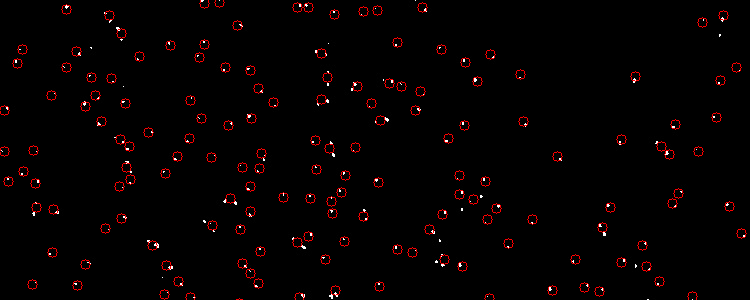
\includegraphics[width=\locateimgsize]{images/locate/trackpy.png}}
	\caption{\centering Trackpy's result}
	\label{fig:locate:trackpy}
\end{figure}

\subsection{Trackpy (CuPy)}

When profiling the Trackpy code, the functions \texttt{fourier\_gaussian}, \texttt{uniform\_filter1d} and \texttt{correlate1d} from \texttt{SciPy} took a considerable amount of time.
For this reason, Trackpy's code was altered to use the \texttt{CuPy} library instead of \texttt{SciPy} for these operations.
This aimed to exploit the GPU for faster computation.

\subsubsection{Algorithm}

The algorithm is the same as Trackpy's, with some extra steps required to transfer the various arrays to/from GPU memory.
These transfers were reduced to the minimum, to reduce the overhead as much as possible.

\subsubsection{Evaluation}

Figure~\ref{fig:locate:trackpy-cupy} shows the result, which for unknown reasons is slightly worse than Trackpy's, at 79\% of identified bubbles.
The algorithm is however faster, running at 7 FPS, but still extremely far from the target.

\begin{figure}
	\centerline{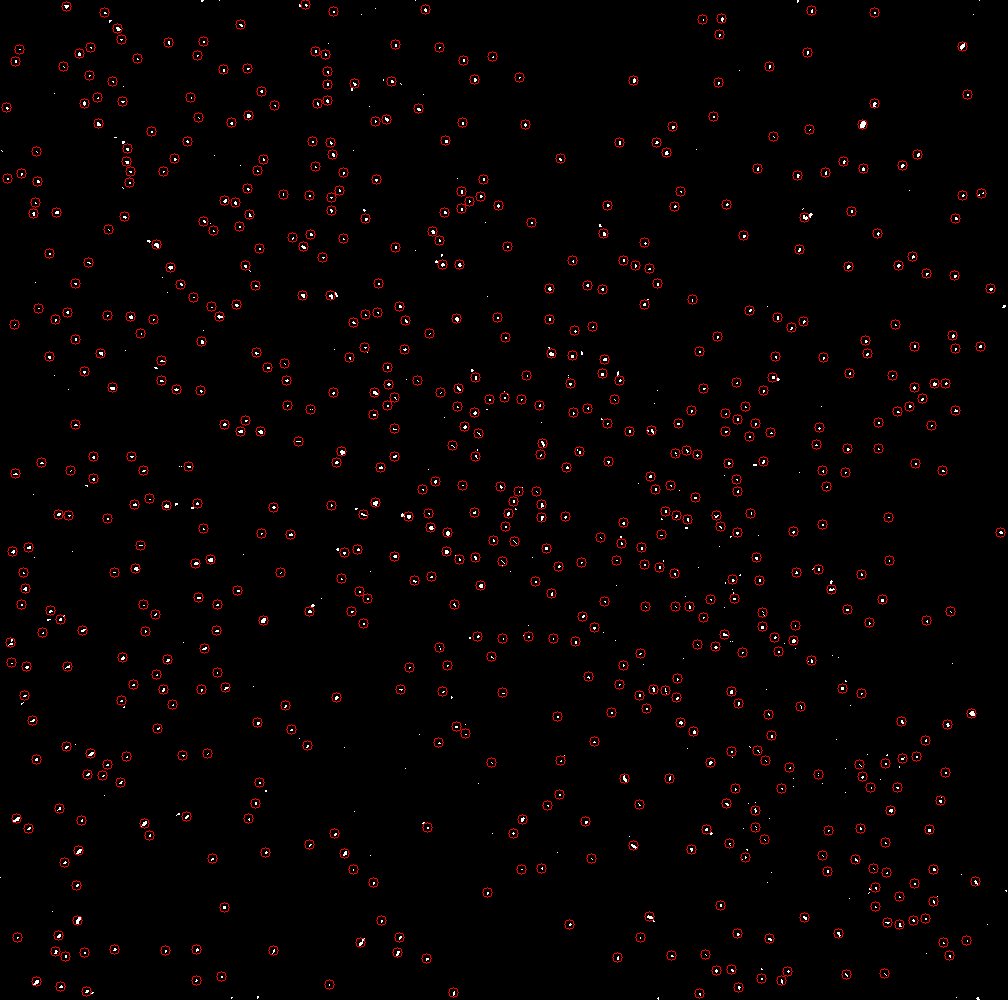
\includegraphics[width=\locateimgsize]{images/locate/cuda-trackpy.png}}
	\caption{\centering Trackpy with CuPy's result}
	\label{fig:locate:trackpy-cupy}
\end{figure}

\subsection{CNN}

The task of \textit{finding the coordinates of the bubbles} can be seen as \textit{for each pixel, check if it is the center of a bubble}.
The task of looking for the same thing across all pixels of an image is the foundation of image convolution and convolutional layers in neural network.
As such, a SAME CONV neural layer was proposed, with a kernel size big enough for containing a full bubble.
The CNN would transform the input image into a binary image, where ``on'' pixels would represent bubble centers.

\subsubsection{Algorithm}

\begin{itemize}
	\itemsep 0em
	\item Initially, the single-layer CNN evaluates the image, to find centroids of the bubbles;
	\item At a second stage, a loop would collect all the ``on'' pixels of the image into a list of coordinates.
\end{itemize}

\subsubsection{Evaluation}

Initially, only a feasibility study was performed: the CNN was trained with just a single epoch of 8 images, to evaluate if the inference speed was good enough to justify a longer training.
The result shown in figure~\ref{fig:locate:cnn} is promising for the little training performed, but it clearly needs more refinement.

Most importantly, the speed was much greater than the previous ones, at 55 FPS, but still far from the target.
As such, further approaches would be evaluated before performing a deeper training, to investigate if a greater speed was achievable.

\begin{figure}
	\centerline{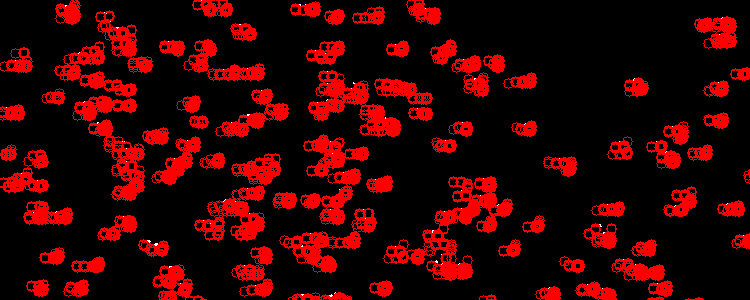
\includegraphics[width=\locateimgsize]{images/locate/cnn.png}}
	\caption{\centering The CNN's result}
	\label{fig:locate:cnn}
\end{figure}

\subsection{...}

...

\subsubsection{Algorithm}

...

\subsubsection{Evaluation}

...

% \begin{figure}
% 	\centerline{\includegraphics[width=\locateimgsize]{images/locate/...}}
% 	\caption{\centering ...'s result}
% 	\label{fig:locate:...}
% \end{figure}


\section{Final choice}
